%%%%%%%%%%%%%%%%%%%%%%%%%%%%%%%%%%%%%%%%%
% Masters/Doctoral Thesis 
% LaTeX Template
% Version 2.5 (27/8/17)
%
% This template was downloaded from:
% http://www.LaTeXTemplates.com
%
% Version 2.x major modifications by:
% Vel (vel@latextemplates.com)
%
% This template is based on a template by:
% Steve Gunn (http://users.ecs.soton.ac.uk/srg/softwaretools/document/templates/)
% Sunil Patel (http://www.sunilpatel.co.uk/thesis-template/)
%
% Template license:
% CC BY-NC-SA 3.0 (http://creativecommons.org/licenses/by-nc-sa/3.0/)
%
%%%%%%%%%%%%%%%%%%%%%%%%%%%%%%%%%%%%%%%%%

%----------------------------------------------------------------------------------------
%	PACKAGES AND OTHER DOCUMENT CONFIGURATIONS
%----------------------------------------------------------------------------------------

\documentclass[
11pt, % The default document font size, options: 10pt, 11pt, 12pt
%oneside, % Two side (alternating margins) for binding by default, uncomment to switch to one side
english, % ngerman for German
singlespacing, % Single line spacing, alternatives: onehalfspacing or doublespacing
%draft, % Uncomment to enable draft mode (no pictures, no links, overfull hboxes indicated)
%nolistspacing, % If the document is onehalfspacing or doublespacing, uncomment this to set spacing in lists to single
%liststotoc, % Uncomment to add the list of figures/tables/etc to the table of contents
%toctotoc, % Uncomment to add the main table of contents to the table of contents
%parskip, % Uncomment to add space between paragraphs
%nohyperref, % Uncomment to not load the hyperref package
headsepline, % Uncomment to get a line under the header
%chapterinoneline, % Uncomment to place the chapter title next to the number on one line
%consistentlayout, % Uncomment to change the layout of the declaration, abstract and acknowledgements pages to match the default layout
]{MastersDoctoralThesis} % The class file specifying the document structure

\usepackage[utf8]{inputenc} % Required for inputting international characters
\usepackage[T1]{fontenc} % Output font encoding for international characters

\usepackage{mathpazo} % Use the Palatino font by default

\usepackage[backend=bibtex,style=authoryear,natbib=true]{biblatex} % Use the bibtex backend with the authoryear citation style (which resembles APA)

\addbibresource{biblio.bib} % The filename of the bibliography

\usepackage[autostyle=true]{csquotes} % Required to generate language-dependent quotes in the bibliography

%----------------------------------------------------------------------------------------
%	MARGIN SETTINGS
%----------------------------------------------------------------------------------------

\geometry{
	paper=a4paper, % Change to letterpaper for US letter
	inner=2.5cm, % Inner margin
	outer=3.8cm, % Outer margin
	bindingoffset=.5cm, % Binding offset
	top=1.5cm, % Top margin
	bottom=1.5cm, % Bottom margin
	%showframe, % Uncomment to show how the type block is set on the page
}

%----------------------------------------------------------------------------------------
%	THESIS INFORMATION
%----------------------------------------------------------------------------------------

\thesistitle{Evaluation of optical aberrations using Phase Diversity} % Your thesis title, this is used in the title and abstract, print it elsewhere with \ttitle
\supervisor{Dr. Laurent \textsc{Jolissaint}} % Your supervisor's name, this is used in the title page, print it elsewhere with \supname
\cosupervisor{Dr. Jean-Paul \textsc{Kneib}}
\examiner{} % Your examiner's name, this is not currently used anywhere in the template, print it elsewhere with \examname
\degree{Master in Applied Physics} % Your degree name, this is used in the title page and abstract, print it elsewhere with \degreename
\author{Jordan \textsc{Voirin}} % Your name, this is used in the title page and abstract, print it elsewhere with \authorname
\addresses{} % Your address, this is not currently used anywhere in the template, print it elsewhere with \addressname

\subject{Optical Physics} % Your subject area, this is not currently used anywhere in the template, print it elsewhere with \subjectname
\keywords{} % Keywords for your thesis, this is not currently used anywhere in the template, print it elsewhere with \keywordnames
\university{\href{http://www.epfl.ch}{Ecole Polytechnique Fédérale de Lausanne}} % Your university's name and URL, this is used in the title page and abstract, print it elsewhere with \univname
\department{\href{http://sb.epfl.ch}{Basic Sciences}} % Your department's name and URL, this is used in the title page and abstract, print it elsewhere with \deptname
\group{\href{http://lastro.epfl.ch/}{Astrophysics laboratory}} % Your research group's name and URL, this is used in the title page, print it elsewhere with \groupname
\faculty{\href{http://sb.epfl.ch/physics}{Physics}} % Your faculty's name and URL, this is used in the title page and abstract, print it elsewhere with \facname

\AtBeginDocument{
\hypersetup{pdftitle=\ttitle} % Set the PDF's title to your title
\hypersetup{pdfauthor=\authorname} % Set the PDF's author to your name
\hypersetup{pdfkeywords=\keywordnames} % Set the PDF's keywords to your keywords
}

\begin{document}

\frontmatter % Use roman page numbering style (i, ii, iii, iv...) for the pre-content pages

\pagestyle{plain} % Default to the plain heading style until the thesis style is called for the body content

%----------------------------------------------------------------------------------------
%	TITLE PAGE
%----------------------------------------------------------------------------------------

\begin{titlepage}
\begin{center}

\vspace*{.06\textheight}
{\scshape\LARGE \univname\par}\vspace{1.5cm} % University name
\textsc{\Large Master Thesis}\\[0.5cm] % Thesis type

\HRule \\[0.4cm] % Horizontal line
{\huge \bfseries \ttitle\par}\vspace{0.4cm} % Thesis title
\HRule \\[1.5cm] % Horizontal line
 
\begin{minipage}[t]{0.4\textwidth}
\begin{flushleft} \large
\emph{Author:}\\
{\authorname} % Author name - remove the \href bracket to remove the link
\end{flushleft}
\end{minipage}
\begin{minipage}[t]{0.4\textwidth}
\begin{flushright} \large
\emph{Supervisors:} \\
\href{https://www.researchgate.net/profile/Laurent_Jolissaint/publications}{\supname}\\ % Supervisor name - remove the \href bracket to remove the link  
\href{https://people.epfl.ch/cgi-bin/people?id=222189&op=bio}{\cosupname}
\end{flushright}
\end{minipage}\\[3cm]
 
\vfill

\large \textit{A thesis submitted in fulfillment of the requirements\\ for the degree of \degreename}\\[0.3cm] % University requirement text
\textit{in the}\\[0.4cm]
\groupname\\\deptname\\[2cm] % Research group name and department name
 
\vfill

{\large \today}\\[4cm] % Date
%\includegraphics{Logo} % University/department logo - uncomment to place it
 
\vfill
\end{center}
\end{titlepage}

%----------------------------------------------------------------------------------------
%	DECLARATION PAGE
%----------------------------------------------------------------------------------------

\begin{declaration}
\addchaptertocentry{\authorshipname} % Add the declaration to the table of contents
\noindent I, \authorname, declare that this thesis titled, \enquote{\ttitle} and the work presented in it are my own. I confirm that:

\begin{itemize} 
\item This work was done wholly or mainly while in candidature for a research degree at this University.
\item Where any part of this thesis has previously been submitted for a degree or any other qualification at this University or any other institution, this has been clearly stated.
\item Where I have consulted the published work of others, this is always clearly attributed.
\item Where I have quoted from the work of others, the source is always given. With the exception of such quotations, this thesis is entirely my own work.
\item I have acknowledged all main sources of help.
\item Where the thesis is based on work done by myself jointly with others, I have made clear exactly what was done by others and what I have contributed myself.\\
\end{itemize}
 
\noindent Signed:\\
\rule[0.5em]{25em}{0.5pt} % This prints a line for the signature
 
\noindent Date:\\
\rule[0.5em]{25em}{0.5pt} % This prints a line to write the date
\end{declaration}

\cleardoublepage

%----------------------------------------------------------------------------------------
%	QUOTATION PAGE
%----------------------------------------------------------------------------------------

\vspace*{0.2\textheight}

\noindent\enquote{\itshape Thanks to my solid academic training, today I can write hundreds of words on virtually any topic without possessing a shred of information, which is how I got a good job in journalism.}\bigbreak

\hfill Dave Barry

%----------------------------------------------------------------------------------------
%	ABSTRACT PAGE
%----------------------------------------------------------------------------------------

\begin{abstract}
\addchaptertocentry{\abstractname} % Add the abstract to the table of contents
The Thesis Abstract is written here (and usually kept to just this page). The page is kept centered vertically so can expand into the blank space above the title too\ldots
\end{abstract}

%----------------------------------------------------------------------------------------
%	ACKNOWLEDGEMENTS
%----------------------------------------------------------------------------------------

\begin{acknowledgements}
\addchaptertocentry{\acknowledgementname} % Add the acknowledgements to the table of contents
The acknowledgments and the people to thank go here, don't forget to include your project advisor\ldots
\end{acknowledgements}

%----------------------------------------------------------------------------------------
%	LIST OF CONTENTS/FIGURES/TABLES PAGES
%----------------------------------------------------------------------------------------

\tableofcontents % Prints the main table of contents

\listoffigures % Prints the list of figures

\listoftables % Prints the list of tables

%----------------------------------------------------------------------------------------
%	ABBREVIATIONS
%----------------------------------------------------------------------------------------

\begin{abbreviations}{ll} % Include a list of abbreviations (a table of two columns)

\textbf{LAH} & \textbf{L}ist \textbf{A}bbreviations \textbf{H}ere\\
\textbf{WSF} & \textbf{W}hat (it) \textbf{S}tands \textbf{F}or\\

\end{abbreviations}

%----------------------------------------------------------------------------------------
%	PHYSICAL CONSTANTS/OTHER DEFINITIONS
%----------------------------------------------------------------------------------------

\begin{constants}{lr@{${}={}$}l} % The list of physical constants is a three column table

% The \SI{}{} command is provided by the siunitx package, see its documentation for instructions on how to use it

Speed of Light & $c_{0}$ & \SI{2.99792458e8}{\meter\per\second} (exact)\\
%Constant Name & $Symbol$ & $Constant Value$ with units\\

\end{constants}

%----------------------------------------------------------------------------------------
%	SYMBOLS
%----------------------------------------------------------------------------------------

\begin{symbols}{lll} % Include a list of Symbols (a three column table)

$a$ & distance & \si{\meter} \\
$P$ & power & \si{\watt} (\si{\joule\per\second}) \\
%Symbol & Name & Unit \\

\addlinespace % Gap to separate the Roman symbols from the Greek

$\omega$ & angular frequency & \si{\radian} \\

\end{symbols}

%----------------------------------------------------------------------------------------
%	DEDICATION
%----------------------------------------------------------------------------------------

\dedicatory{For/Dedicated to/To my\ldots} 

%----------------------------------------------------------------------------------------
%	THESIS CONTENT - CHAPTERS
%----------------------------------------------------------------------------------------

\mainmatter % Begin numeric (1,2,3...) page numbering

\pagestyle{thesis} % Return the page headers back to the "thesis" style

% Include the chapters of the thesis as separate files from the Chapters folder
% Uncomment the lines as you write the chapters

% Chapter 1

\chapter*{Introduction} % Main chapter title
\addcontentsline{toc}{chapter}{Introduction}
\label{Introduction} % For referencing the chapter elsewhere, use \ref{Chapter1} 

%----------------------------------------------------------------------------------------

% Define some commands to keep the formatting separated from the content 
\newcommand{\keyword}[1]{\textbf{#1}}
\newcommand{\tabhead}[1]{\textbf{#1}}
\newcommand{\code}[1]{\texttt{#1}}
\newcommand{\file}[1]{\texttt{\bfseries#1}}
\newcommand{\option}[1]{\texttt{\itshape#1}}

%----------------------------------------------------------------------------------------

This master thesis treats one of the major challenges in astronomy and in optics in general, the aberrations and their corrections. We will study and develop a method to identify the static aberrations present in an  optical system using the data produced by it.

\vspace{1cm}


Ground based observation is as old as the first men. But since the Galilei Galileo telescope in 1609, the resolution power of the telescopes is far greater. Many inventions lead to the construction of the largest telescope ever built, the Very Large Telescope (VLT). Now that we are able to build enormous telescopes with mirror diameter up to 8m, soon to be bitten by the Extremely Large Telescope (ELT) with its 18m primary mirror diameter, the limitation of the resolution is not the diameter anymore, but the inhomogeneities of the Earth's atmosphere. Indeed, the turbulence present in the atmosphere creates a turbulent distribution of refractive index due to the distribution of temperature principally. This alters the optical path of the light through the atmosphere which finally deteriorates the images given by the telescope.

\begin{figure}
\begin{center}
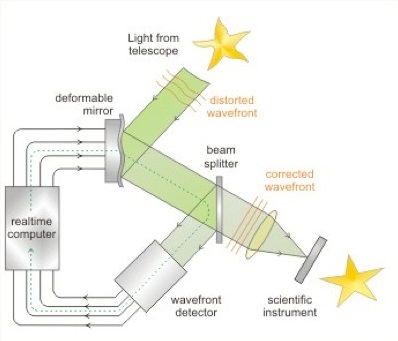
\includegraphics[width=0.6\textwidth,angle=0]{Figures/ao_scheme.jpg}
\caption{Adaptive optics schema}
source : Institut National of Astrophysics, Bologna Observatory, 2018, \url{http://www.bo.astro.it/ter5/ter5/ao.html}.
\label{fig:ao_scheme}
\end{center}
\end{figure}

In the 1980's, systems to correct aberrations in telescopes called an active optics system were developed. It consists of actuators placed under the telescope mirrors capable of correcting the telescope deformation due to the effect of wind, temperature, gravity, vibration, etc... Those systems works at  around 1 Hz , which is not fast enough to correct for the turbulence of the atmosphere (100-1000 Hz) but they are essential in the construction of large telescopes. The state-of-the-art technique is the adaptive optics, developed to take into account the effects of the atmosphere. This technique monitors the aberrations present in the wavefront and corrects them in real time. The schema of principle is shown in Figure \ref{fig:ao_scheme}. It uses a wavefront sensor to characterize its deformation and then passes the information to a deformable mirror to correct it. It is called an adaptive optic loop. It works well, but the drawback of this method is that it does not correct the aberrations up to the scientific detector. Those uncorrected aberrations are called Non-Common Path Aberration (NCPA), they are generally static or slowly evolving over time. The adaptive optic also requires a complex optical system before the scientific detector. The beam is split in two parts. One arm goes to the scientific detector and the other is used in the adaptive optic loop.

We present here a method called phase diversity that uses images of the scientific detector to deduct the aberrations present in the wavefront. In our case, the phase diversity is used to correct the static aberrations that deform the wavefront. Our work is inspired by the phase diversity idea that was first introduced by \citet{Gonsalves_1982}. The idea is to use one focused and one defocused image to retrieve the aberrations. Two images at least are needed due to the property of light acquisition. There is an indetermination, because the detector is only sensitive to the intensity of light and not the light wave itself. This indetermination is raised adding a phase diversity. Unlike adaptive optic system, the phase diversity requires nearly no additional optical component depending on how it is implemented. The final aim of this project would be to integrate the developed phase diversity into the design of the DAG (Dogu Anadolu Gozlemevi) telescope in Turkey, see Figure \ref{fig:DAGtelescope}.

\begin{figure}
\begin{center}
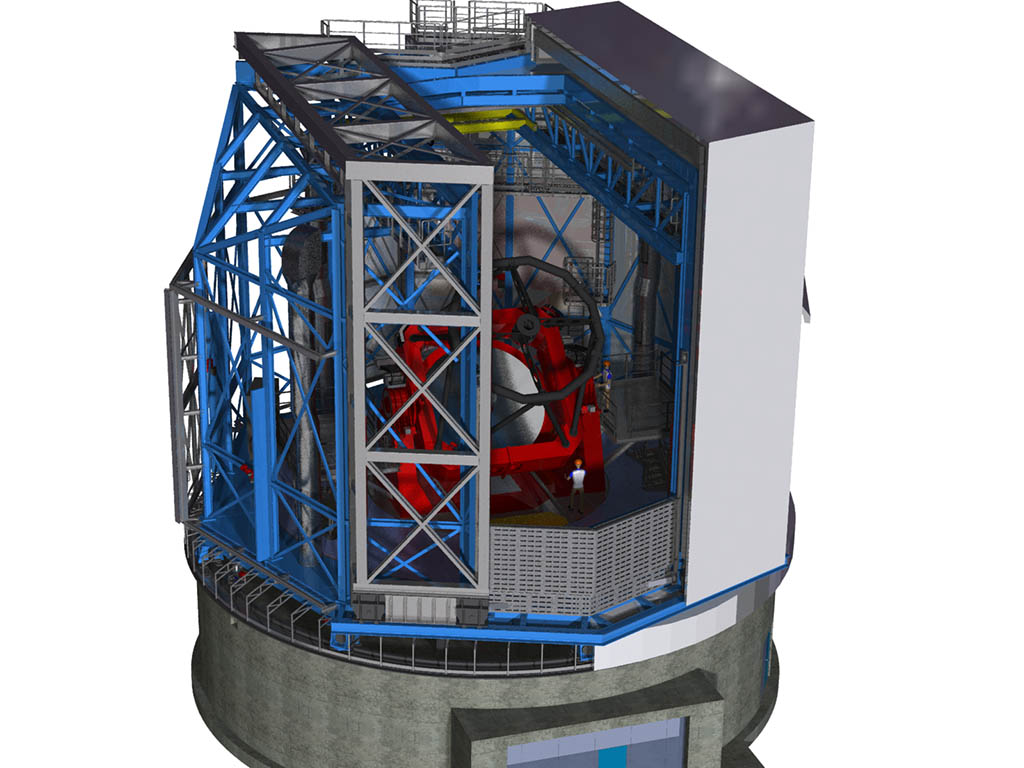
\includegraphics[width=0.5\textwidth,angle=0]{Figures/DAGtelescope.jpg} \\
\caption{DAG 4m telescope} 
source : EIE group, 2018, \url{http://www.eie.it/en/progetti/dag-dogu-anadolu-gozlemevi}.
\label{fig:DAGtelescope}
\end{center}
\end{figure}

\vspace{1cm}

This report is organized in three main chapters. First, a review of the necessary theoretical background is reminded, going from the scalar theory of diffraction to the description of phase retrievals methods. Then we present an experiment performed at the optic laboratory at HEIG-VD. The ONERA (Office National d'Etudes et de Recherches Aerospatiales) algorithm of phase diversity is tested and used in comparison with a Shack-Hartmann wavefront sensor. And finally, the development of an analytical phase diversity algorithm is presented and tested with simulated Point Spread Functions (PSFs).

\chapter{Phase Diversity Experiment} 
\label{ch:PDExp}

Here, we will describe the experiment put in place in the optical laboratory at the HEIG-VD to reconstruct wavefronts with unknown static aberrations introduced using phase screens. At first, we study the  behaviour of the phase diversity algorithm put in place by \citet{mugnier_2006} at ONERA with respect to number of averaging images, in other words noise level, and number of Zernike coefficients retrieved. Then we test the algorithm using a known aberration introduced by a parallel plane plate in the beam comparing the result to Zemax simulation. And finally, we introduce the phase screen to have random aberrations in the pupil and try to compare the phase diversity results with the Shack Hartman wavefront sensor results.

\section{Experimental Setup}
\label{sec:ExpSetup}
\begin{figure}
\begin{center}
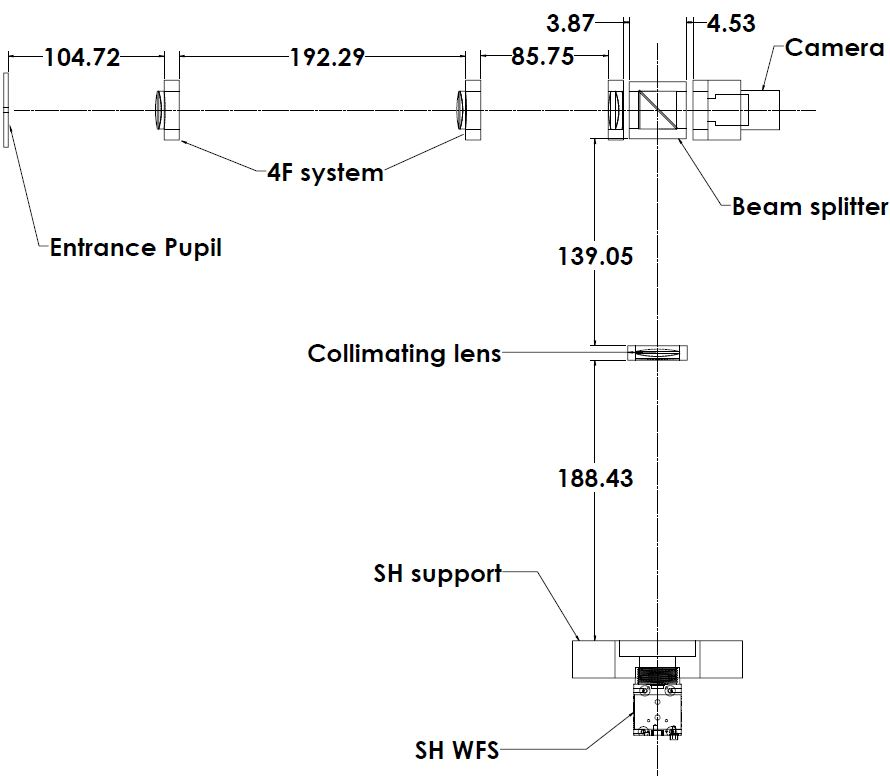
\includegraphics[width=0.8\textwidth,angle=0]{Figures/setupSchema.JPG}
\decoRule
\caption[Experimental Setup Schema]{Experimental setup schema with the relevant distances, \citep{Bouxin_PDM}.}
\label{fig:setupSchema}
\end{center}
\end{figure}

The design of the experiment was already done by \citet{Bouxin_PDM}. The system is built according to her plans and specifications. Figure \ref{fig:setupSchema} shows the schema of the experimental setup.

The experiment is mounted on a pressurized legs optical table. The assembly contains six main components : a light source, an entrance pupil, an imaging system, a converging lens to focus the beam on the camera, a camera and a wavefront sensor.

\subsection{Light source}
\label{subsec:LigthSource}

\begin{minipage}{\linewidth}
\begin{wrapfigure}{r}{0.4\textwidth}
\centering
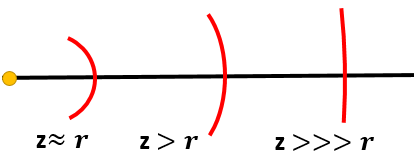
\includegraphics[width=0.4\textwidth]{Figures/WFdistantSource.PNG}
\decoRulewrapFig
\caption[Wavefront curvature]{Wavefront curvature for different point source's distances, \textit{z}. \textit{r} represents the characteristic size of the arc of interest.}
\label{fig:WFdistantSource}
\end{wrapfigure}

The final application of the phase diversity will be to characterize the optical aberrations induced by the imperfect optical path to a scientific detector of a telescope. For this reason, the light source has to simulate a distant star aberration-free wavefront. A distant star wavefront is considered planar since the object distance, z, is far greater than the telescope size, r, see Fig. \ref{fig:WFdistantSource}. The source of our experiment must then be characterized by a planar wavefront.

In order to obtain such a planar wavefront at the entrance pupil, the light source consist of a "pigtailed laser diode", a f=11mm converging lens, a pinhole and a f=200 mm converging lens, see Table \ref{tab:optComp}. The pigtailed laser diode emits a Gaussian beam centred at 637.5 nm slightly diverging. The converging lens concentrates the beam at the center of the 10$\mu$m pinhole to filter the noise. The second converging lens collimates the beam, obtaining a collimated beam with a planar wavefront, see Fig. \ref{fig:sourceRayTracing} and \ref{fig:pinholeEffect}.

\end{minipage}

\begin{figure}
\centering
    \begin{subfigure}{0.5\textwidth}
        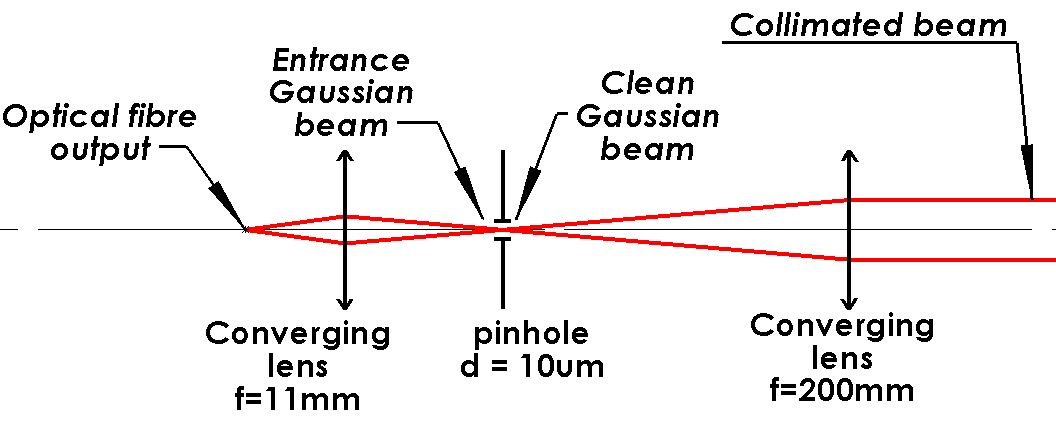
\includegraphics[width=\textwidth]{Figures/source.png}
        \caption{Source ray tracing.}
        \label{fig:sourceRayTracing}
    \end{subfigure}
    \quad
    \begin{subfigure}{0.3\textwidth}
        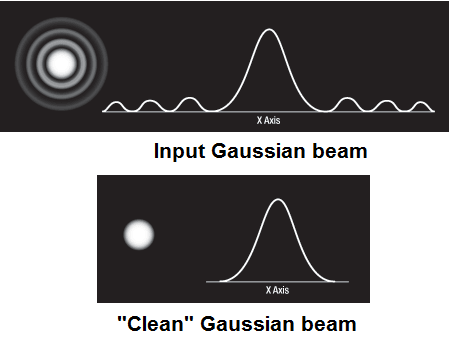
\includegraphics[width=\textwidth]{Figures/pinholeEffect.png}
        \caption{Beam view before and after the pinhole, \citep{SpatialFilters}.}
        \label{fig:pinholeEffect}
    \end{subfigure}
    \decoRule
    \caption{Source schema and pinhole effect on the beam.}
\end{figure}

\subsection{Entrance pupil}
\label{subsec:EntrancePupil}

The entrance pupil of our optical system is a circular aperture of 3.2 mm diameter placed after the collimating lens of the light source. It is milled in a metal plate and centred in his support, to avoid positioning with a XY table. The diameter is chosen in available material to fit in the different detector's surfaces.

\subsection{Pupil imaging system}
\label{subsec:pupilImSystem}

The phase diversity technique requires PSFs images as input, which means that the beam as to be focused onto the detector surface. To analyse the aberration in the pupil plane, one needs to focus an image of the beam passing through the entrance pupil. The simplest assembly to achieve this goal is the 4F system, which consist of two converging lenses of focal 100 mm. The two lenses are separated by 200 mm, see Fig. \ref{fig:setupSchema}. This places the image of the entrance pupil 100 mm after the second converging lens.

\subsection{Detectors}
\label{subsec:Detectors}

The image of the entrance pupil, obtained with the 4F system, is focused onto a CMOS Ximea camera by a f = 80 mm converging lens to acquire the PSFs for the phase diversity wavefront retrieval. The camera has a surface composed by 1280x1024 pixels of 5.3 $\mu$m, see Appendix \ref{app:ximeaCam}. It is mounted on sliding support in order to be able to acquire in/out-of-focus images. A beam splitter is placed in the converging beam to separate it in two. The second beam is collimated and a Shack-Hartman WFS is placed on the entrance pupil image plane, to check the results of the phase diversity wavefront retrieval. The Shack-Hartman WFS has a 39 X 31 lenslets grid and a CCD with a resolution of 1280x1024 pixels of 4.65 $\mu$m, see Appendix \ref{app:SHwfs}. 

\begin{table}
\caption{Optical Components}
\label{tab:optComp}
\centering
\begin{tabular}{|l|l|l|c|}
\hline
\textbf{\#}& \textbf{Components} & \textbf{Model} & \textbf{Reference} \\\hline
1 & Pigtailed laser diode & Thorlabs, LPS-635-FC & \ref{app:pigtailedLaserDiode} \\\hline
2 & Converging lens, f = 11 mm & Thorlabs, A220TM-A & \ref{app:CL11} \\\hline
3 & Pinhole, 10 $\mu$m & Thorlabs, P10S & \ref{app:pinhole10microns} \\\hline
4 & Converging lens, f = 200 mm & Thorlabs, AL100200 & \ref{app:CL200} \\\hline
5 & 3.2 mm Hole milled in metal sheet & ... & ... \\\hline
6 & Converging lens, f = 100 mm & Thorlabs, AC254-100-A & \ref{app:CL100} \\\hline
7 & Converging lens, f = 80 mm & & \\\hline
8 & Camera CMOS & Ximea, MQ013MG-E2 & \ref{app:ximeaCam} \\\hline
9 & Converging lens, f = 100 mm & & \\\hline
10 & Shack-Hartman WFS & Thorlabs, WFS150-5C & \ref{app:SHwfs} \\\hline
\end{tabular}
\end{table}

\section{Data Acquisition}
\label{sec:DataAcquis}

\subsection{Ximea Camera}
\label{subsec:acquisXimCam}

The ONERA algorithm takes at least one focused and one defocused PSFs, as described in section \ref{subsec:OneraAlgoImp}. The PSFs are acquired using a python script which uses an open-source library to control the ximea camera, \verb|pyXimea|\footnote{\url{https://github.com/pupil-labs/pyximea}}, available on GitHub. The acquisition is done following these steps : 

\begin{enumerate}

\item The first step in order to acquire PSFs is to determine the position of the camera's focus point using the python script \verb|AlignementScriptXimeaCamera.py|, see Appendix \ref{subapp:AlignementScriptXimeaCamera}. This script let's you acquire consecutively PSFs at different camera's positions and computes their FWHM. It finally returns the minimum FWHM and the camera's position, see Figure \ref{subfig:28092017AlignementXimeaPSFs} and \ref{subfig:28092017AlignementXimeaPos}.

\begin{figure}
\centering
    \begin{subfigure}{\textwidth}
        \includegraphics[width=\textwidth]{../../../fig/alignement/28092017AlignementXimeaPSFs.png}
        \caption{PSFs taken during the alignment procedure, each image is taken at an other camera position.}
        \label{subfig:28092017AlignementXimeaPSFs}
    \end{subfigure}
    \\
    \begin{subfigure}{0.6\textwidth}
        \includegraphics[width=\textwidth]{../../../fig/alignement/28092017AlignementXimeaPos.png}
        \caption{FWHM of the PSFs as a function of the camera's position. The minimum is at $11.55$ mm}
        \label{subfig:28092017AlignementXimeaPos}
    \end{subfigure}
    \decoRule
    \caption{Example of the results of an alignment procedure}
\end{figure}

\item Once the focus point position of the camera is determined, the acquisition of the data is possible. The acquisition script is called \verb!AcquisAndSaveXimea.py!, see Appendix \ref{subapp:AcquisAndSaveXimea}.

\item The user needs to set the main parameters before acquiring. They are the number of images on which to average, the size of the final PSFs, the position of the focus point on the sliding system and the initial guess to fit the 2D Gaussian on the PSF to find its center. The initial guess can be made using the Ximea camera software, called \verb!xiCamTool!, with which one gets a live feedback of the camera.

\item Then the running program ask the user what he needs to do after having made a sound. The first thing the user needs to do is to place the camera at the focus point and turn on the LED in order to set the optimal exposure time in order to avoid saturation.

\item Finally the acquiring sequence begins, the program ask the user to shut down and turn on the source as the user acquire the different images to get the dark images and the PSF images. The user needs to manually displace the camera to get the defocused PSFs. The program computes the positions to get a $2\pi$ P2V defocus dephasing.

\end{enumerate}

Many functions, used in the two scripts described above, are coded in the script \verb!functionsXimea.py!, see Appendix \ref{subapp:functionsXimea}.

\subsection{Shack-Hartmann WFS}
\label{subsec:acquisSHwfs}

The Shack-Hartmann wavefront sensor acquisition is done with the company software. The acquired data are the Zernike coefficients and the reconstructed wavefront computed following the principle described in section \ref{subsec:SHprinciple}. Their is a few parameters that the user can set : the exposure time (there is also an auto set), the number of averaging images (1 up to 300) and the focus points reference of the micro-lenses array. 

The data are saved manually in a \textit{.csv} file. I coded an IDL script to read and average the Shack-Hartmann data, in order to be able to analyse them and compare the result with the phase diversity, see Appendix \ref{subapp:readAndAverageSHdata} and \ref{subapp:readSHWFSdata}. 

\section{Results}
\label{sec:Results}

This section presents the results of the phase diversity experiment, with the introduction of different sources of aberration. We will first present the results of the ONERA algorithm test, then we will compare the phase diversity retrieval with a calibrated aberration and finally we will introduce random static aberration with the phase screen and compare the results to the Shack-Hartmann wavefront sensor results.

\subsection{ONERA Phase Diversity test}
\label{subsec:ONERAPDtest}

The motivation of this test was to better understand the behaviour of the ONERA phase diversity algorithm with respect to the different parameters that could influence its results, such as the noise present in the PSFs, the number of Zernike coefficients returned for the modal mode and the error on the defocused distance of the PSFs.

\begin{figure}
\begin{center}
\includegraphics[width=0.6\textwidth,angle=0]{../../../fig/PD/noise_study/NoiseCurveXimea}
\decoRule
\caption{Noise level as a function of the number of averaging images acquired with $\sim$ 300 $\mu$s exposition time. The noise level is computed as the mean of the standard deviation of every pixel divided by the maximum of the focused PSF.}
\label{fig:NoiseCurve}
\end{center}
\end{figure}

To study the noise, we acquire PSFs with 25 different numbers of averaging images going from 10 to 5000. The noise level is computed as the ratio between the mean pixel standard deviation and the PSF maximum. The Ximea detector has a noise curve visible in Figure \ref{fig:NoiseCurve}. The noise curve is computed with the noise level of the focused PSFs. It follows an exponential law with the number of averaging images. The noise level varies from $\sim 1\mathrm{e}-3$ to $\sim 8\mathrm{e}-5$, for 10 and 5000 images respectively. Having the noise curve of the detector, we can study empirically how it influences the phase diversity results. 

\begin{figure}
\centering
    \begin{subfigure}{0.8\textwidth}
        \includegraphics[width=\textwidth]{../../../fig/PD/noise_study/ZernikeCoef_J_differentNbrAveraging.png}
        \caption{Zernike coefficients $a_j$ as a function of $j$ the Zernike index of the 25 modal and zonal phase retrievals, in blue and red respectively.}
        \label{subfig:ZernikeCoef_J_differentNbrAveragingjmax30}
    \end{subfigure}
    \\
    \begin{subfigure}{0.5\textwidth}
        \includegraphics[width=\textwidth]{../../../fig/PD/noise_study/Boxplot_Aj_j_jmax30.png}
        \caption{Boxplot of the 25 Zernike coefficients $a_j$ of the different phase retrievals computed with the different averaging numbers of images as a function of the Zernike index $j$.}
        \label{subfig:Boxplot_Aj_j_jmax30}
    \end{subfigure}
    \decoRule
    \caption{Results of the phase retrievals computed with the 25 different noise levels. The phase retrievals are done with a $j_{max} = 30$}
\end{figure}

Figures \ref{subfig:ZernikeCoef_J_differentNbrAveragingjmax30} and \ref{subfig:Boxplot_Aj_j_jmax30} presents the results of the 25 different retrievals. As one can see there is some spread due to the different noise levels present in the PSFs given to the algorithm. The biggest standard deviation on a Zernike coefficient is smaller than 6 nm. And there can be up to 20 nm of maximal difference between the $a_j$'s as one can see on Figure \ref{subfig:Boxplot_Aj_j_jmax30}. The spherical aberration, $a_{11}$, has the biggest standard deviation and range of values. This shows that the PSFs noise levels have an impact on the retrieval and that not all Zernike coefficient are affected in the same way. One reassuring point is the good correspondence between the modal and zonal retrievals.

\begin{figure}
\begin{center}
\includegraphics[width=\textwidth,angle=0]{../../../fig/PD/noise_study/WavefrontsNoiseStudy}
\decoRule
\caption{Reconstructed wavefronts for two different number of averaging images, 10 and 3500, left and right column respectively. The two first line are modal retrieval with $j_{max}=30$ and $j_{max}=200$ and the last line is the zonal retrieval.}
\label{fig:WavefrontsNoiseStudy}
\end{center}
\end{figure}

Furthermore, looking at the reconstructed wavefronts in Figure \ref{fig:WavefrontsNoiseStudy}, one can see the effect of noise in the PSFs and how important is the choice of $j_{max}$ for the modal reconstruction. Indeed, for the wavefronts reconstructed using $j_{max}=30$, the retrieved structures are similar, however for $j_max=200$ there are more structures in the retrieval done on the PSFs with 10 averaging images. This shows that the noise has a signal at high spatial frequencies. The zonal retrieval shows it clearly, the reconstruction is significantly different between 10 and 3500 averaging images. The averaging over a large number of acquisition smooth out the noise structures that perturbs the reconstruction. Also as said above with the Zernike coefficients is still valid for the wavefront, the two retrieval method gives similar results. But Figure \ref{fig:WavefrontsNoiseStudy} shows that the choice of $j_{max}$ is important if one wants to use the reconstructed wavefronts.

\newpage
\subsection{Parallel plane plate}
\label{subsec:ParPlanePlate}

The first source of aberration studied in this work is a tilted parallel plane plate which is used as a calibrated source of astigmatism.
 
%\include{Chapters/Chapter3}
%\include{Chapters/Chapter4} 
%\include{Chapters/Chapter5} 

%----------------------------------------------------------------------------------------
%	THESIS CONTENT - APPENDICES
%----------------------------------------------------------------------------------------

\appendix % Cue to tell LaTeX that the following "chapters" are Appendices

% Include the appendices of the thesis as separate files from the Appendices folder
% Uncomment the lines as you write the Appendices

% Appendix A

\chapter{Optical Component Datasheets}
\label{AppendixA} 

\section{Pigtailed laser diode}

\includepdf[pages=-,width=\textwidth]{../../componentDatasheet/LPS-635-FC-SpecSheet.pdf}

%\include{Appendices/AppendixB}
%\include{Appendices/AppendixC}

%----------------------------------------------------------------------------------------
%	BIBLIOGRAPHY
%----------------------------------------------------------------------------------------

\printbibliography[heading=bibintoc]

%----------------------------------------------------------------------------------------

\end{document}  
